O HeapSort é um eficiente algoritmo de ordenação que se baseia no conceito de árvores binárias, especificamente na estrutura de dados conhecida como Heap. Desenvolvido em 1964 por Robert W. Floyd e J.W.J. Williams, este método compartilha a Ordem de Complexidade O(n log n) com outros algoritmos eficientes, mas se distingue pelo uso de heaps para otimizar o processo de seleção dos itens.\cite{mello2002ordenacao}

Funcionamento do HeapSort:
O processo do HeapSort inicia com a construção de um heap, que pode ser um heap máximo (max heap) ou mínimo (min heap). Em um max heap, cada nó pai tem um valor maior que o de seus filhos, enquanto em um min heap, cada nó pai tem um valor menor. Isso coloca o maior (ou menor) valor na raiz da árvore, que corresponde ao primeiro elemento do array.\cite{lopes2005heap}

O algoritmo então repete o processo de remoção do nó raiz (o maior ou menor elemento, dependendo do tipo de heap), reposicionando o último elemento do heap na raiz e reajustando a estrutura para manter as propriedades do heap. Esse processo de reajuste, ou "heapify", é essencial para manter a ordem correta durante a ordenação.

 \begin{figure}[H]
    \centering
    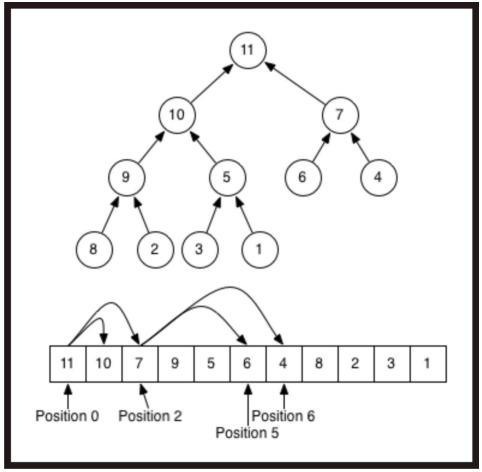
\includegraphics[width = 6cm]{Imagens/Heap Sort/image.png}
    \caption{Ilustração de um Heap máximo\cite{lopes2005heap}. }
    \label{imagem_heap}
\end{figure}

Os algoritmos para implementar as operações sobre o heap operam ao longo de um dos caminhos da árvore, a partir da raiz até o nível mais profundo da árvore. Para o HeapSort, são necessárias apenas duas operações com o heap: \textit{Remake}, que refaz a estrutura, e \textit{Build}, que a constrói. Eles são apresentados no Programa 1.

\begin{verbatim}
Programa 1: Operações com Heap necessárias ao HeapSort.
void SortMethods::ReMake(long Left, long Right, TItem *Array) {
    long i = Left;
    long j;
    TItem aux;
    j = i * 2;
    aux = Array[i];
    while (j <= Right) {
        if (j < Right) {
            this->mComparations++;
            if (Array[j].Key < Array[j + 1].Key)
                j++;
        }
        this->mComparations++;
        if (aux.Key >= Array[j].Key)
            break;
        Array[i] = Array[j];
        i = j;
        j = i * 2;
        this->mMoviments++;
    }
    Array[i] = aux;
    this->mMoviments++;
}

void SortMethods::Build(TItem *Array, long n) {
    long Left;
    Left = n / 2 + 1;
    while (Left > 1) {
        Left--;
        ReMake(Left, n, Array);
    }
}
\end{verbatim}

O método de Ordenação HeapSort é iniciado com um heap obtido através do método \textit{Build}.

\begin{verbatim}
Programa 2: Método HeapSort.
void SortMethods::HeapSort(TItem *Array, long n) {
    long Left, Right;
    TItem aux;
    CTimer *Timer = new CTimer();
    this->ClearAll();
    Timer->start();
    this->Build(Array, n);
    Left = 0;
    Right = n-1;
    while (Right > 0) {
        aux = Array[0];
        Array[0] = Array[Right];
        Array[Right] = aux;
        this->mMoviments++;
        Right--;
        this->ReMake(Left, Right, Array);
    }
    Timer->stop();
    this->mTime = Timer->getElapsedTime();
}
\end{verbatim}

Depois pega-se o item na posição 0 do vetor(raiz do heap) e troca-se com o
item que está na posição n do vetor, como apresentado no Programa 2. A seguir,
basta usar o método ReMake com o restante dos itens. A Figura 29\ref{fig:imagem_heap1} ilustra o
funcionamento deste método.

 \begin{figure}[H]
    \centering
    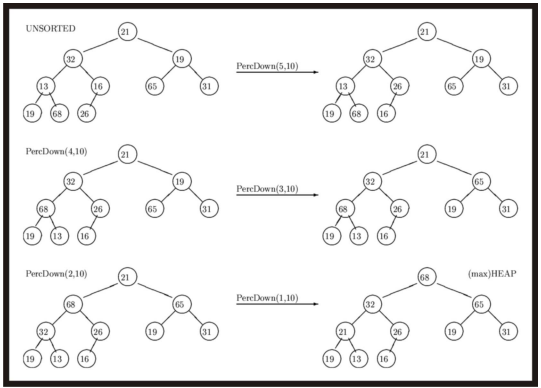
\includegraphics[width = 6cm]{Imagens/Heap Sort/heapheao.png}
    \caption{Ilustração do funcionamento do algoritmo HeapSort. }
    \label{imagem_heap1}
\end{figure}

